%!TEX TS-program = xelatex

%%%%%%%%%%%%%%%%%%%%%%%%%%%%%%%%%%%%%%%%%%%%%%%%
% CV template
%  created by muhammad farhan
%%%%%%%%%%%%%%%%%%%%%%%%%%%%%%%%%%%%%%%%%%%%%%%%
\documentclass[]{cv-class}
\usepackage{afterpage}
\usepackage{fancyhdr}
\usepackage{hyperref}
\usepackage{fontawesome5}
\RequirePackage[hidelinks]{hyperref}
\hypersetup{
    pdftitle={MuhammadFarhan-CV},
    pdfauthor={engr.farhan@icloud.com},
    pdfsubject={Muhammad Farhan Key Technology Expert},
    pdfkeywords={},
    colorlinks=true,           % no lik border color
    allbordercolors=white       % white border color for all
}
\fancyhf{}
\fancyhfoffset{0em}
% Remove head rule
\renewcommand{\headrulewidth}{0pt}
%\fancyfoot[C]{\thepage}
\pagestyle{fancy}
\newcommand*{\makecvfooter}[3]{%
  \fancyfoot{}
  \fancyfoot[L]{#1}
  \fancyfoot[C]{#2}
  \fancyfoot[R]{#3}
}
% \begin{flushright} - \emph{\today}
% \end{flushright}
\usepackage{color}
\usepackage{amssymb}% to access $\blacksquare$
\newcommand{\ctag}[1]{%
  \tikz[baseline]\node[anchor=base,draw=white!70,rounded corners=0.5ex,inner xsep=1ex,inner ysep =0.55ex,text height=1.3ex,text depth=.25ex]{#1};
}
\newcommand{\ptag}{\ctag{\color{darkGrey!70} $\blacksquare$}}

\newcommand{\btag}{\ctag{\color{red!70} $\blacksquare$}}
\newcommand{\mtag}{\ctag{\color{pblue!70} $\blacksquare$}}
\newcommand{\mobileSymbol}{\faPhone}
\newcommand{\itag}[1]{%
  \tikz[baseline]\color{accent!80}\node[anchor=base,draw=darkGrey!70,rounded corners=1.5ex,inner xsep=1ex,inner ysep =0.55ex,text height=1.3ex,text depth=.25ex]{#1};
}

\newcommand{\cvtag}[1]{%
  \tikz[baseline]\color{accent!80}\node[anchor=base,draw=darkGrey!70,rounded corners=1.5ex,inner xsep=1ex,inner ysep =0.55ex,text height=1.3ex,text depth=.25ex]{#1};
}
\newcommand{\stag}[1]{%
  \tikz[baseline]\color{accent!80}\node[anchor=base,draw=darkGrey!70,rounded corners=1.0ex,inner xsep=1ex,inner ysep =0.55ex,text height=1ex,text depth=.25ex]{#1};
}
\newcommand{\sociallink}[3]{\mbox{\textcolor{gray}{#1}\hspace{0.5em}\link{#2}{#3}\hspace{1em}}}
\newcommand*{\email}[1]{\sociallink{\mailSymbol}{mailto:#1}{#1}}
\newcommand*{\smartphone}[1]{\sociallink{\mobileSymbol}{tel:#1}{#1}}    
\usepackage{xcolor}
\hypersetup{
    colorlinks=true,
    linkcolor=blue
}
\addbibresource{bibliography.bib}
\RequirePackage{xcolor}
\definecolor{pblue}{HTML}{0395DE}
\begin{document}

% \fancyhead{} % clear all header fields

\header{Muhammad}{Farhan}
      {Agile Projects - Quality Assurance- Devops- Full-Stack Development}

% Fake text to add separator
\vspace{1.15cm}
\fcolorbox{white}{gray}{\parbox{\dimexpr\textwidth-2\fboxsep-2\fboxrule}{%
.....
}}




% In the aside, each new line forces a line break
\begin{aside}
  
\includegraphics[scale=0.40]{img/pic.jpg}
    ~
  \vspace{0.65cm}
  \section{Martial status}
    Married
  	~
  \section{Address}
    House#253 Eden Cottages Phase-1, \\ Lahore 
    Pakistan
    ~
  \section{Phone}
 {+92 300 4028200}
  \section{Mail}
    \underline{\href{mailto:engr.farhan@icloud.com}{engr.farhan@icloud.com}}
    ~
  \section{Web}
  	%\underline{\href{http://martinothamar.github.io}{martinothamar.github.io}}
	\vspace{0.10cm}
    \underline{\href{https://www.linkedin.com/in/engr-farhan}{\faLinkedin LinkedIn}}
	\vspace{0.10cm}\\
    \underline{\href{https://hub.docker.com/r/intigration/}{\faDocker Docker}}
	\vspace{0.10cm}\\
    \underline{\href{https://github.com/intigration}{\faGithub GitHub}}
	\vspace{0.10cm}\\
    \underline{\href{https://codepen.io/intigration}{\faCodepen CodePen.io}}
    ~
  % \section{Programming}
  %   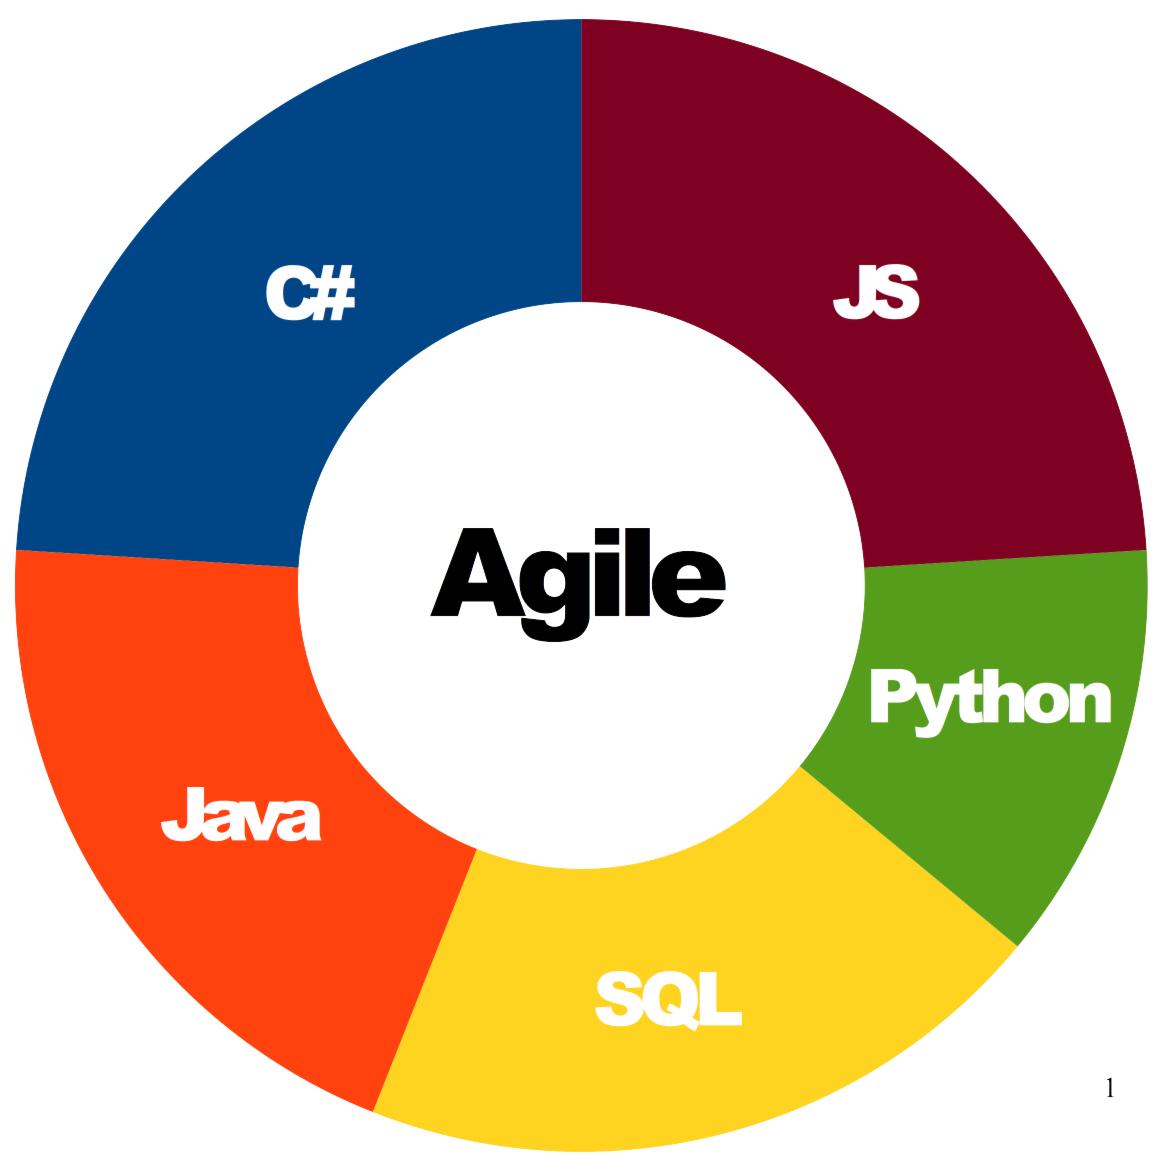
\includegraphics[scale=0.22]{img/programming.png}
    ~
  \section{ \underline{Expertise}}
{\small
\itag{$\blacksquare$ Quality \& Process Governance}\\
\vspace{2mm}
\itag{$\blacksquare$ Scripting \& Automation}\\
\vspace{2mm}

\itag{$\blacksquare$ Communication Skills} \\
\vspace{2mm}

\itag{$\blacksquare$ Organizational Skills}\\
\vspace{2mm}

\itag{$\blacksquare$ CI \& CD}\\
\vspace{2mm}

\itag{$\blacksquare$ Office365,Project \& ALM tooling chain }  \\
\vspace{2mm}

\itag{$\blacksquare$ Agile Retrospective,Sprint mgmnt \& Backlog} \\
\vspace{2mm}
\itag{$\blacksquare$ AI and Machine Learning Usecases}\\\vspace{2mm}

\itag{$\blacksquare$ Blockchain,Identity mgmnt \& Databases}\\
\vspace{2mm}

\itag{$\blacksquare$ {CyberSecurity} \& \\{TRA}}\\
\vspace{2mm}

  \itag{$\blacksquare$ API Integration \& Microservices}\\
  \vspace{2mm}



\itag{$\blacksquare$ Test planning \& management}\\
\vspace{2mm}

\itag{$\blacksquare$ SOA \& Distributed Systems}
\vspace{2mm}
}\\
    \asidelist{\textbf{JavaScript}}
    {
\includegraphics[scale=0.30]{img/star.png}
    
\includegraphics[scale=0.30]{img/star.png}
    
\includegraphics[scale=0.30]{img/star.png}
    
\includegraphics[scale=0.30]{img/star.png}
    
\includegraphics[scale=0.30]{img/star.png}}\\
    \asidelist{\textbf{Python}}
    {
\includegraphics[scale=0.30]{img/star.png}
    
\includegraphics[scale=0.30]{img/star.png}
    
\includegraphics[scale=0.30]{img/star.png}
    
\includegraphics[scale=0.30]{img/star.png}
    
\includegraphics[scale=0.30]{img/star_empty.png}}\\
    \asidelist{\textbf{Bash/Lua }} 
    {
\includegraphics[scale=0.30]{img/star.png}
    
\includegraphics[scale=0.30]{img/star.png}
    
\includegraphics[scale=0.30]{img/star.png}
    
\includegraphics[scale=0.30]{img/star.png}
    
\includegraphics[scale=0.30]{img/star_empty.png}}\\
   
  % \section{Places lived}
    % \includegraphics[scale=0.62]{img/norway.png}

  % \section{Languages}
  %   \asidelist{\textbf{Norwegian}}
  %   {
\includegraphics[scale=0.30]{img/star.png}
  %   
\includegraphics[scale=0.30]{img/star.png}
  %   
\includegraphics[scale=0.30]{img/star.png}
  %   
\includegraphics[scale=0.30]{img/star.png}
  %   
\includegraphics[scale=0.30]{img/star.png}}
  %   \asidelist{\textbf{English}}
  %   {
\includegraphics[scale=0.30]{img/star.png}
  %   
\includegraphics[scale=0.30]{img/star.png}
  %   
\includegraphics[scale=0.30]{img/star.png}
  %   
\includegraphics[scale=0.30]{img/star.png}
  %   
\includegraphics[scale=0.30]{img/star_empty.png}}
  %   \asidelist{\textbf{Faroese}}
  %   {
\includegraphics[scale=0.30]{img/star.png}
  %   
\includegraphics[scale=0.30]{img/star.png}
  %   
\includegraphics[scale=0.30]{img/star_empty.png}
  %   
\includegraphics[scale=0.30]{img/star_empty.png}
  %   
\includegraphics[scale=0.30]{img/star_empty.png}}
  %   \asidelist{\textbf{German}}
  %   {
\includegraphics[scale=0.30]{img/star.png}
  %   
\includegraphics[scale=0.30]{img/star_empty.png}
  %   
\includegraphics[scale=0.30]{img/star_empty.png}
  %   
\includegraphics[scale=0.30]{img/star_empty.png}
  %   
\includegraphics[scale=0.30]{img/star_empty.png}}


% \cvtag{ $\blacksquare$ \textbf{DevOps, Containerization, Kubernates }}
% \cvtag{ $\blacksquare$ \textbf{IoT Edge \& Device Management}} 

% \begin{itemize}
%     \item Technology \& Innovation (TI)
%     \begin{itemize}
%              \item Reference Application Design (RAD)
%     \item Technology Transfer (TT)
%     \end{itemize}
%     \item Process Quality Management  (TQM)
%         \item   Operations \& Deployment (DevOps) 
%      \item Validation (VAL) \begin{itemize}
%      \item Quality Assurance \& System Test  (QA)
%           \item Field Test \& Deployment (FTD)
%      \end{itemize}
%      \item Project Management Office (PMO)
%      \item Product Management Group (PMG)
%      \item System Level Engineering (SLE)
%      \begin{itemize}
%          \item Cloud Application Services (CAS)
%          \item Cloud Services Platform (CSP)
%          \item Industrial Edge (IE)
%          \item Embedded System Design (ESD)  
%     \end{itemize}
%      \item Autonomous Factory (AF)
%      \begin{itemize}
%           \item Industrial AI Systems 
%      \end{itemize}
% \end{itemize}



\end{aside}
% \vspace{0.75cm}
\section{Summary}

        \item {
\includegraphics[scale=0.30]{img/star.png}} An \textbf{enthusiastic} about making technology purposeful and sell-able
           \item {
\includegraphics[scale=0.30]{img/star.png}} Full \textbf{Remote} compliant infra, secured network, power backup and extended tooling
        \item {
\includegraphics[scale=0.30]{img/star.png}}  Member of Active Tax payer \& Engineering Council (PEC) \textbf{ELECTRO /12552}
        \item {
\includegraphics[scale=0.30]{img/star.png}} Proven track record with extensive working experience in every SDLC stage.
             \item {
\includegraphics[scale=0.30]{img/star.png}} Ready environments \& Speedy resolutions to common SDLC challenges
        \item {
\includegraphics[scale=0.30]{img/star.png}} Sustainable planning through lean \& \textbf{specialized risk suppression} techniques
        \item {
\includegraphics[scale=0.30]{img/star.png}} {\textbf{ PMI-Agile Certified Petitioner} - Project Management Institute (Training)}
        \item {
\includegraphics[scale=0.30]{img/star.png}} \textbf{Simplifying AI technology} adoption for human \& business both
  
        \item {
\includegraphics[scale=0.30]{img/star.png}}{\textbf{ Mind-Sphere Applications Developer }Workshop (Onsite: Erlangen, Germany) }
        \item {
\includegraphics[scale=0.30]{img/star.png}} \textbf{Won awards} and appreciation letters from Senior Management at SIEMENS, MGC \& Intech process Automation on various occasions for showing excellent performance.
        \item {
\includegraphics[scale=0.30]{img/star.png}}{\textbf{ ISTQB® CTFL}- 2016-CTFL-00101-PK International Testing Qualifications Board}
        \item {
\includegraphics[scale=0.30]{img/star.png}} \textbf{Innovation} through \textbf{modern} tooling, agility, \textbf{openness} \& delegation.
        \item {\includegraphics[scale=0.30]{img/star.png}}\textbf{Transparency}: zero waste approach, Modular Design, Re-usability
        \item {\includegraphics[scale=0.30]{img/star.png}} culture of appreciation, \textbf{respect everyone's} opinion
        \begin{itemize}
            \item {\includegraphics[scale=0.30]{img/star.png}} \textbf{Improve continuously}, achieved goals \& established collective success
        \end{itemize}
          \textbf{$\bigstar$}  I combine \textbf{vision with operational, domain \& technical expertise}  to bring next-generation technologies to market in record time.\\
 % \end{quote}
 \vspace{1mm}

                 \wheelchart{1.2cm}{0.4cm}{
             18/6em/pblue!40/ Programming languages \&\\ Scripting,
              20/6em/pblue!80/DevOps \& Kubernates\\ Virtualization,
              40/6em/pblue!90/PLM Management \& Release Operations, 
             10/6em/pblue!30/Penetration \& NFR \\ Testing,
              22/6em/pblue!45/System Integration \&\\ Automation
        }
    \vspace{3mm} 
            { \textbf{Extensive} \textbf{working} experience in overall PLM functions.Led productization process to ensure the product is built according to standard process gates (criteria) of planning, development and deployment}\\
                                      $\blacksquare$ Product Portfolio evaluation\\
                                       $\blacksquare$ Cybersecurity\\
                                       $\blacksquare$ Project planning\\
                                       $\blacksquare$ Solution validation\\
                                       $\blacksquare$ Project Risk classification\\
                                       $\blacksquare$ OSS Clearance\\
                                       $\blacksquare$ Technology patents\\
                                       $\blacksquare$ Service offering, pricing \& Licensing\\
                                       $\blacksquare$ EHS and all other legal or compliance relevant topics\\
\section{Highlights}
Please see the highlights for operational defectiveness in deliverable.

\begin{aside}
    \section{ \underline{Functional Areas}}
    \vspace{2mm}
   Here are my common high level functionality and my daily work aspects :\\ 
    \vspace{2mm} \faCheck Resources capability retention, development \& training \\
  \vspace{2mm} \faCheck MVP \& quick Prototyping \\

  \vspace{2mm} \faCheck Test cases development \& execution \\
  \vspace{2mm} \faCheck use-cases identification \& translation \\
  \vspace{2mm} \faCheck Functional,integration \& NFR test environment management \\
\vspace{2mm} \faCheck Health Checks, release pipelines \& Workflows \\
\vspace{2mm} \faCheck Quality \& release metrics tracking and implementation \\ \vspace{2mm}

\vspace{2mm} \faCheck Autonomous \& Data Intelligence Systems \\
\vspace{2mm} \faCheck IoT \& Service delivery model (SaaS) \\
\vspace{2mm} \faCheck System Simulation techniques \& Test Methods \\
\vspace{2mm} \faCheck Cloud infra \& Virtualization \\
\vspace{2mm} \faCheck Quality governance \& PL \\
\vspace{2mm} \faCheck Codebase configuration management \\
\vspace{2mm} \faCheck Project dependencies \& computability \\
\vspace{2mm} \faCheck Data Simulation sources \& Backing services \\
\vspace{2mm} \faCheck Release Build, release, deploy workflows \\
\vspace{2mm} \faCheck Infra Concurrency, Disposability, Dev/prod parity (Environments) \\ 

                 \vspace{2mm} \faCheck Delivery definition \& new offerings: continuously validate new business offering with existing product/projects \\
             \vspace{2mm} \faCheck Cloud strategies \&  SaaS  management \\
        \vspace{2mm} \faCheck Test Logs \& Management reporting \\
        \vspace{2mm} \faCheck Running Experiments \\

  

\end{aside}
        \textbf{$\blacksquare$ Deployment Frequency Increase} Elevated the deployment frequency from a monthly to a weekly or daily release cycle, leading to faster feature delivery and increased agility.\\
         \textbf{$\blacksquare$ Deployment Success Rate} Achieved a consistently high success rate for deployments, with <10\% fewer rollbacks or failed deployments over a specific period.\\
         \textbf{$\blacksquare$ Reduced Downtime} Minimized downtime during deployments, resulting in a significant reduction in system unavailability and improved product and testing service reliability.\\
        \textbf{$\blacksquare$ Automation Percentage} Increased the percentage of automated tasks in the CI/CD pipeline by 75\%, reducing manual intervention and accelerating the release process.\\
         \textbf{$\blacksquare$ Mean Time to Recovery (MTTR)} Reduced the MTTR for incidents, ensuring faster incident resolution and less impact on users.\\
        \textbf{$\blacksquare$ Infrastructure as Code (IaC)} Adoption Implemented IaC practices, resulting in a less dependant infrastructure provisioning pipeline and decreased configuration-related errors.\\
        \textbf{$\blacksquare$ OPC DA 2.0 and AE 1.01 Certification} for IntelliMAX OPC DA Server and A\&E Server.
       \begin{itemize}
       \item  \textbf{IntelliMAX OPC DA and AE }clients interoperatabilty
       \item  \textbf{IntelliMAX Historian} - ZERO Data Loss: To guarantee that there is end to end ZERO\% data loss when IntelliMAX is deployed in a \textbf{distributed} architecture. The data includes VTQs (from PLC) and ‘Alarms Generation’ inside IntelliMAX. The challenge is to communicate the huge flux across the client Server chains and store it inside the server.
       \item  Designed and Executed Stress, Load, Data loss Validation, Sanity and Regression tests
       \item  Launched BETA and Commercial product releases i.e. \textbf{simulating plant environment} in lab using PLCs from following vendor. Allen-Bradley, Modicon, SCADA PACK and GE
       \item  \textbf{Benchmark}'d IntelliMAX Data Historian with OSIsoft PI (Stress Testing) - Data Archiving and Data Retrieval on trends
       \end{itemize}
   \\
         \textbf{$\blacksquare$ Implementation of Tech-Support frame work} to establish the level of responsibility among the groups, expected response time commitments, and when to appropriately escalate an issue and to which level? This framework is also supported to diagnose and resolve common problems typically going through the exact same past problems by managing history / knowledge-base.\\
       \textbf{$\blacksquare$ Resource Cost Optimization} Lowered infrastructure costs by Xthrough efficient resource allocation, auto-scaling, and cost monitoring.\\
   \textbf{$\blacksquare$ Security Vulnerabilities Mitigation} Decreased the number of security vulnerabilities in production through automated scanning, patching, and proactive security measures.\\
     \textbf{$\blacksquare$ Monitoring and Alerting Improvements} Enhanced monitoring and alerting systems, resulting less false positives and faster incident detection.\\
   \textbf{$\blacksquare$  Microsoft Test Manager} was implemented within existing infrastructure to facilitate the testers and developers for better organization and execution strategies for their test plans, also improved tester effectiveness, reliability, and repeatability. Test Cases design and review activities were integrated with Team foundation server.\\
    	$\blacksquare$ Established\textbf{ QA infrastructure} with the implementation of virtual environments, use of data archiving techniques and provision of necessary hardware’s and software to replicate the production environments.\\
    	$\blacksquare$ \textbf{Visibility to higher management}/stake holders was much increased by providing the multiple Dashboards and status reports to device the present and future strategies.\\
    	$\blacksquare$ Design of \textbf{Product data sheets, }performance bench-marking and redefinition of the artifacts for acceptance and entry/exit criteria for different phases in software development cycle.\\
      \textbf{$\blacksquare$ Cross-Team Collaboration} Facilitated collaboration between development, operations, and other teams, leading to a increase in overall team productivity.\\
         \textbf{$\blacksquare$ Containerization Benefits} Achieved a significant reduction in resource utilization and improved scalability by containerizing applications and services.\\
         \textbf{$\blacksquare$ Compliance Adherence} Ensured compliance with industry standards or regulatory requirements (e.g., HIPAA, GDPR) with zero major compliance violations over a specified period.\\
    \textbf{$\blacksquare$ Infrastructure Resilience} Increased infrastructure resilience by implementing disaster recovery and failover mechanisms, resulting in fewer unplanned outages.\\
         \textbf{$\blacksquare$ Feedback Loop Optimization} Shortened the feedback loop between development and operations teams, resulting in faster issue resolution and improved collaboration.\\
         \textbf{$\blacksquare$ Documentation and Knowledge Sharing} Established comprehensive documentation and knowledge-sharing practices, resulting in reduced onboarding time for new team members.
\section{Education}
\cvevent{\black \textbf{BSc\ in Electronics Engineering}}{\href{https://www.nfciet.edu.pk/}{NFC Institute of Engineering \& Technology}}{2003 -- 2007}{Multan, PK}
    {   {\vspace{2mm} \faCheck}  }{ \textbf{Grade: A+}\newline {\vspace{2mm} \faCheck} \textbf{Professional Engineer} License holder PEC# 12552 \newline Physics and other sciences, applied research, design of devices, equipment, and systems for manufacture, field-testing, the establishment of quality control standards, supervision of manufacture and production testing, and engineering management
}

\begin{aside}
  \vspace{1cm}
  \section{ \underline{Applications}}
  \vspace{2mm}
The list of applications grouped by domain that I worked: \\
  % \section{Places lived}
\vspace{1mm}
    % \includegraphics[scale=0.62]{img/norway.png}
\underline{\textbf{{\color{pblue!70}\faCloud} IoT Cloud & Big Data}}\\
\vspace{2mm}
   \mtag{Device Provisioning}\\
    \mtag{Remote Device Configuration}\\
    \mtag{Firmware OTA Updates}\\
    \mtag{Monitoring and Diagnostics}\\
    \mtag{Security and Access Control}\\
    \mtag{Scalability Lifecycle}\\
    \mtag{Device Grouping and Tagging}\\
     \mtag{Alerts and Notifications}\\
     \mtag{Data Storage and Analytics}\\
     \mtag{Energy Management}\\
     \mtag{Asset Management}\\
     \mtag{Predictive Maintenance}\\
     \mtag{Environmental Monitoring}\\
     \mtag{Process Automation}\\
     \mtag{Healthcare Medical Devices}\\
     \vspace{1mm}
     \underline{\textbf{{\color{red!70}\faBrain} AI \& Machine Learning}}\\
     \vspace{2mm}
      \btag{Computer Vision}\\
       \btag{Speech Recognition}\\
    \btag{Recommendation Systems}\\
    \btag{Autonomous Systems}\\
    \btag{Predictive Analytics}\\
    \vspace{1mm}
\underline{\textbf{{\color{darkGrey!70}\faSignal} \hspace{1mm} SCADA and HMI}}\\
\vspace{2mm}
  \ptag{Plant Information management system}\\
  \ptag{SCADA Historian} \\
  \ptag{Visual HMI Systems}\\
\ptag{Remote Device Telemetry data}\\
\ptag{Alarms \& Event Management}\\
\ptag{MES - Manufacturing Execution Systems}\\
    

 
\end{aside}

\section{Experience}
\cvevent{\underline{  \includegraphics[scale=0.3]{sie.png} |  PLM Officer / System Integration Expert }}{\href{https://www.siemens.com/global/en/company/stories/industry/ai-in-industries.html}{Industrial AI \& Machine Learning}\textbf{ | Digital Industries Factory Automation}}{Aug 22 - Sep 23}{ Hybrid, Lahore}

Led the overall QA activities for the AI and ML software product line which involves numerous GA product releases and various services projects\\
     $\blacksquare$ Develop and manage project plans for different product releases, test automation and services projects\\
     $\blacksquare$ Consultation, coordination and collaboration within QA and with development teams and marketing\\
     $\blacksquare$ Project progress, defects tracking, QA metrics and status reporting, issues resolution and risks identification\\
     $\blacksquare$ Product requirements analysis and maintain traceability matrices
     Projects execution and resources management\\
     $\blacksquare$ Test coverage analysis and test cases review\\
     $\blacksquare$ Test automation frameworks design and implementation\\
     $\blacksquare$ Processes development, implementation and improvements\\
     $\blacksquare$ Correspondence on issues with development teams and customers\\
     $\blacksquare$ Documentation/code/design reviews\\
        \cvtag{ $\blacksquare$ \textbf{Team Management}}
        \cvtag{ $\blacksquare$ \textbf{Delivery Flow Acceleration}}
        \cvtag{ $\blacksquare$ \textbf{Office 365 Tooling}}\\
        \cvtag{ $\blacksquare$ \textbf{PLM Management}} 
        \cvtag{ $\blacksquare$ \textbf{Continuous Integration}}
        \cvtag{ $\blacksquare$ \textbf{Kubeflow}}
        \cvtag{ $\blacksquare$ \textbf{AWS}}
    
\cvevent{ \underline{\includegraphics[scale=0.3]{sie.png} | Senior Technical Lead}}{\href{https://plm.sw.siemens.com/en-US/insights-hub/} {Industrial Operations X } | MindSphere Industrial IoT Cloud }{Aug 17 - Sep 22}{Hybrid, Lahore}

    { Played a key role in executing on the IoT Software Platform test automation strategy, driving quality and testability of built over AWS}\\ 
                 { $\blacksquare$ Enabled integrated collaboration env, work visibility for technology development teams}\\
                 { $\blacksquare$  PLM milestones planning \& quality gate qualification criteria's.}\\
                 { $\blacksquare$ Standardization in release workflows \& adopted tooling }\\
                 { $\blacksquare$ Process tunning \& documentation.}\\  
    $\blacksquare$ Built and tested highly scalable mesh network, where distributed services run in public, private and hybrid cloud infrastructures\\
    { $\blacksquare$ Defined defect tracking and correction procedures, monitoring and updating defect reports as needed}\\
    { $\blacksquare$ Wrote test scripts to assess software quality, and develops automated test reporting to increase test effectiveness.}\\
    { $\blacksquare$ Developed test plans and test procedures for testing of all components at the unit, module, system and integration levels, performing risk analysis when required.}\\
    { $\blacksquare$ Built and test large scale messaging infrastructure, data replication}
 
                  
    

       
\cvtag{ $\blacksquare$ \textbf{NodeRed}}           
\cvtag{ $\blacksquare$ \textbf{Polarion}}
\cvtag{ $\blacksquare$ \textbf{Microsoft Altassian Tooling}}
\cvtag{ $\blacksquare$ MachineLearning}
\cvtag{$\blacksquare$ Edge Applications}
\cvtag{$\blacksquare$ AWS-Hybrid Cloud}
\cvtag{$\blacksquare$ AWS-Lambda}\\
\cvtag{$\blacksquare$ AWS-GreenGrass}
\cvtag{$\blacksquare$ sqlite}
\cvtag{$\blacksquare$ Angular}\cvtag{$\blacksquare$ Linux Runtime \& Containers}

            

\begin{aside}
\section{\underline{Tooling Chain}}
{\Huge
 \faAws \hspace{1mm}\faNode \hspace{1mm}\faJenkins \\
 \faPython \hspace{1mm}  \faLinux \hspace{1mm} \faGitlab \\
 \faConfluence \hspace{1mm} \faJira \hspace{1mm}   \faPhp \\
 \faReact \hspace{1mm} \faNodeJs \hspace{1mm} \faDocker \\ 
 \faGit \hspace{1mm} \faGitlab \hspace{1mm} \faMarkdown \\
 \faRaspberry


}
    \section{ \underline{Organizations}}
    Here is the list of organizations that I worked for: \\
{\small \begin{itemize}
    \item Technology \& Innovation (TI)
    \begin{itemize}
             \item Reference Application Design (RAD)
    \item Technology Transfer (TT)
    \end{itemize}
    \item Process Quality Management  (TQM)
        \item   Operations \& Deployment (DevOps) 
     \item QA \& Validation \begin{itemize}
     \item System Test  (SYS)
          \item Field Test \& Deployment (FTD)
     \end{itemize}
     \item Project Management Office (PMO)
     \item Product Management Group (PMG)
     \item System Level Engineering (SLE)
     \begin{itemize}
         \item Cloud Application Services (CAS)
         \item Cloud Services Platform (CSP)
         \item Industrial Edge (IE)
         \item Embedded System Design (ESD)  
    \end{itemize}
     \item Autonomous Factory (AF)
     \begin{itemize}
          \item Industrial AI Systems 
     \end{itemize}
     
\end{itemize}
}
\end{aside}                     
\cvevent{ \underline{\includegraphics[scale=0.15]{mentor.jpg}{ | Senior Technical Lead}}}{\href{https://www.linkedin.com/company/mentor/products/}{Cloud Services Platform}{ (SLE)}}{Apr 15 - Aug 17}{OnSite, Lahore}

The required acceleration to speeds up technology innovation requires both technical domain expertise \& tailored process framework.\\$\blacksquare$  Led QA activities for cloud and embedded software product line\\
    $\blacksquare$ Product requirements analysis\\
    $\blacksquare$ Test coverage analysis, test cases development and review\\
    $\blacksquare$ Develop and manage test plans for different product releases\\
    $\blacksquare$ Test plans execution\\
    $\blacksquare$ Test automation, test frameworks design and implementation\\
    $\blacksquare$ Documentation reviews\\
    $\blacksquare$ Processes development, implementation and improvements\\
    $\blacksquare$ Project status reporting \\

\cvtag{ $\blacksquare$ MQTT, IoT Protocols}
\cvtag{ $\blacksquare$ Data Simulation} 
\cvtag{ $\blacksquare$ Cloud Connectors}
\cvtag{ $\blacksquare$ Virtual Devices }
\cvtag{ $\blacksquare$ Postman, ReadyAPI}
\cvtag{ $\blacksquare$ Embedded Devices Testing}
              
\newpage
\cvevent{ \includegraphics[scale=0.1]{2018030209315414145.jpg} | Delivery Compliance \& QA Manager}{\href{https://www.intechwww.com}{Intech Process Automation Inc}}{June 2009 -- April 2015}{OnSite, Lahore PK}
    $\blacksquare$ Innovated sellable quality product\\
    $\blacksquare$ Acted central point for development, architects, documentation, PMG, Commercial, services and Enterprise quality.\\
    $\blacksquare$ Led the teams of software testers and field test engineers to build the validation strategies for mission critical and fault tolerant industrial systems and applications.\\
  $\blacksquare$  Built agreements, guidelines, and standards in order to resolve issues and create practices.\\
 $\blacksquare$  Respect people.Talent hunt and resource training.\\
    \cvtag{ $\blacksquare$ OPCUA}
    \cvtag{ $\blacksquare$ ISA95}
        \cvtag{ $\blacksquare$ SCADA}
    \cvtag{ $\blacksquare$ Distributed Systems}
        \cvtag{ $\blacksquare$ Performance Testing}
        \cvtag{ $\blacksquare$ JMETER}
        \cvtag{ $\blacksquare$ Regression Test}

\cvevent{\includegraphics[scale=0.2]{imperious (1).jpg}{Applications Engineer}}{\href{https://www.imperioustech.com}{Imperious Technologies}}{September 2007 -- June 2009}{OnSite, Lahore,PK}
\begin{itemize}
    \item Delivered commercial complaint criteria and control strategy for the products under test
    \item Assisted development process for faster production grade release.

\end{itemize}

\section{References}
\begin{aside}
    \section{\underline{Projects}}
    Projects details can be seen at \underline{\href{https://www.linkedin.com/in/engr-farhan/details/projects/}{LinkedIn}}
    \vspace{2mm}
        \item $\blacksquare$ Machine Learning and Flow Manager (Framework to develop AI apps)
        \item $\blacksquare$ ORION - (Machine learning model traning runtime)
        \item $\blacksquare$ IntelliMAX (Industrial Automation \& HMI Software)
        \item $\blacksquare$ CSP - Cloud Services Platform
        \item $\blacksquare$ Distributed Intelligence
        \item $\blacksquare$ IoT Device Management
        \item $\blacksquare$ M3 - Machine Monitoring \& Management
        \item $\blacksquare$ OEE (Overall equipment efficiency)
        \item $\blacksquare$ OPC server \& client compliance DA/HDA/AnE
        \item $\blacksquare$ PLC Alarming
        \item $\blacksquare$ Plant Assets Ontology ISA95
        \item $\blacksquare$ Plant Information Management System - SCADA Historian
        \item $\blacksquare$ Product security Cyber threat \& risk assessment
        \item $\blacksquare$ SCADA hot redundant Server \& Client Switchover
        \item $\blacksquare$ Simulation Twin Lab
        \item $\blacksquare$ Transfer of Technology - JV
    \end{aside}
\begin{entrylist}
The references are taken from \underline{\href{https://www.linkedin.com/in/engr-farhan/details/recommendations/}{LinkedIn recommendation section}}\\
\includegraphics[scale=0.5]{Testimonials.png}
\end{entrylist}

\vspace{1cm}
\begin{flushright}
If you need more personal, professional and reference details. It can be provided upon the request. please don't hesitate to contact me\\
Yours sincerely,\\
\emph{Muhammad Farhan}
\end{flushright}
	\makecvfooter
		{Last Updated \textsc{\underline{\textbf{\today}}}} % \selectlanguage{english}\today
		{\textsc{\underline{\href{mailto:engr.farhan@icloud.com}{Muhammad Farhan}}}}
		{\href{}{Source Code} \hspace{2mm}Total Pages:\thepage}





\end{document}